% English draft based on sections/05_emergent_stopping_layer_ja.tex
\section{The Emergent Stopping Layer $L_E$}

\noindent\textbf{Scope of the account.} The inference, log, and stopping layers are model-local functional roles, not a completed dynamical implementation. Calling a layer a stopping attractor does not establish its existence or explain independently observed stopping. Existence, convergence, and detection independent of stopping behavior remain open. The four-stage account is a qualitative mechanism hypothesis; its arrows supply neither an update law nor a convergence result.

The external stopping operator is an architectural proposal. Its type, relation to iterated inference, and implementation by the stopping layer are unresolved. The external reference field and inter-individual network are compared as two proposed views of shared reference. The printed identity sign is retained, but literal identity and typed isomorphism are not established. Refinement of the Part I potential into a network is likewise proposed, not implemented.

The three profiles retain their examples but do not independently verify autonomous emergence or endogenous mobility. The distinction between a Transformer's own stopping layer and a whole-system external stop remains unresolved; the figure does not decide it. Projection is a role comparison with the consciousness paper, not transfer of the same operator. Stability is not truth, and recoverability/revisability is a proposed functional relation rather than a guarantee.

The active architectural account distinguishes a tracked retention support (described here as RetentionSupport) from a role assessment, a regime, and a process of using it; it does not posit a particular memory store or a new kind of entity. LR and LE, and the temporary scaffold regime explained below, are role descriptions relative to a declared analytical scope and time window. Each assessment identifies the support and its continuity, system and environment sides, feedback recipient, re-reference and transformation paths, criterion, and evidence, or records what is Unknown. Matching content or a name does not establish support identity. A model-supported assessment, a conditional assignment, non-support under a specified criterion, and Unknown are distinct: missing or conflicting information is not absence, falsehood, inaccessibility, or a not-LE judgment.

Ownness is used only as a descriptive bundle of feedback direction and persistence, recipient, re-reference control, reuse, and effects on current state, surfaced history, update conditions, and external structure. It is not a score, binary owner, legal title, subject, or autonomy test. Analytical sides do not fix an ontological subject boundary. The retained diagrams, observed stopping, and the old no-fixed-point argument cannot certify these roles. The active LR and LE paragraphs below supply the current descriptive account; the locally enclosed definitions and mechanisms preserve their historical proposals without making the whole paper archival or denying its other interpretations.


This chapter is the second center of the paper. The historical local-state model in \S{}3 discussed the conditional fixed-point limit of $L_F$ under its stated premises. This chapter proposes a stopping architecture involving the log layer $L_R$ and the emergent stopping layer $L_E$.

Throughout this chapter, inference-F and no-fixed-point references derived from Section 3 refer to that historical model, not the active record/position contract. The later architecture remains a proposal, not a consequence proved by the new interfaces.

\begin{figure}[H]
\centering
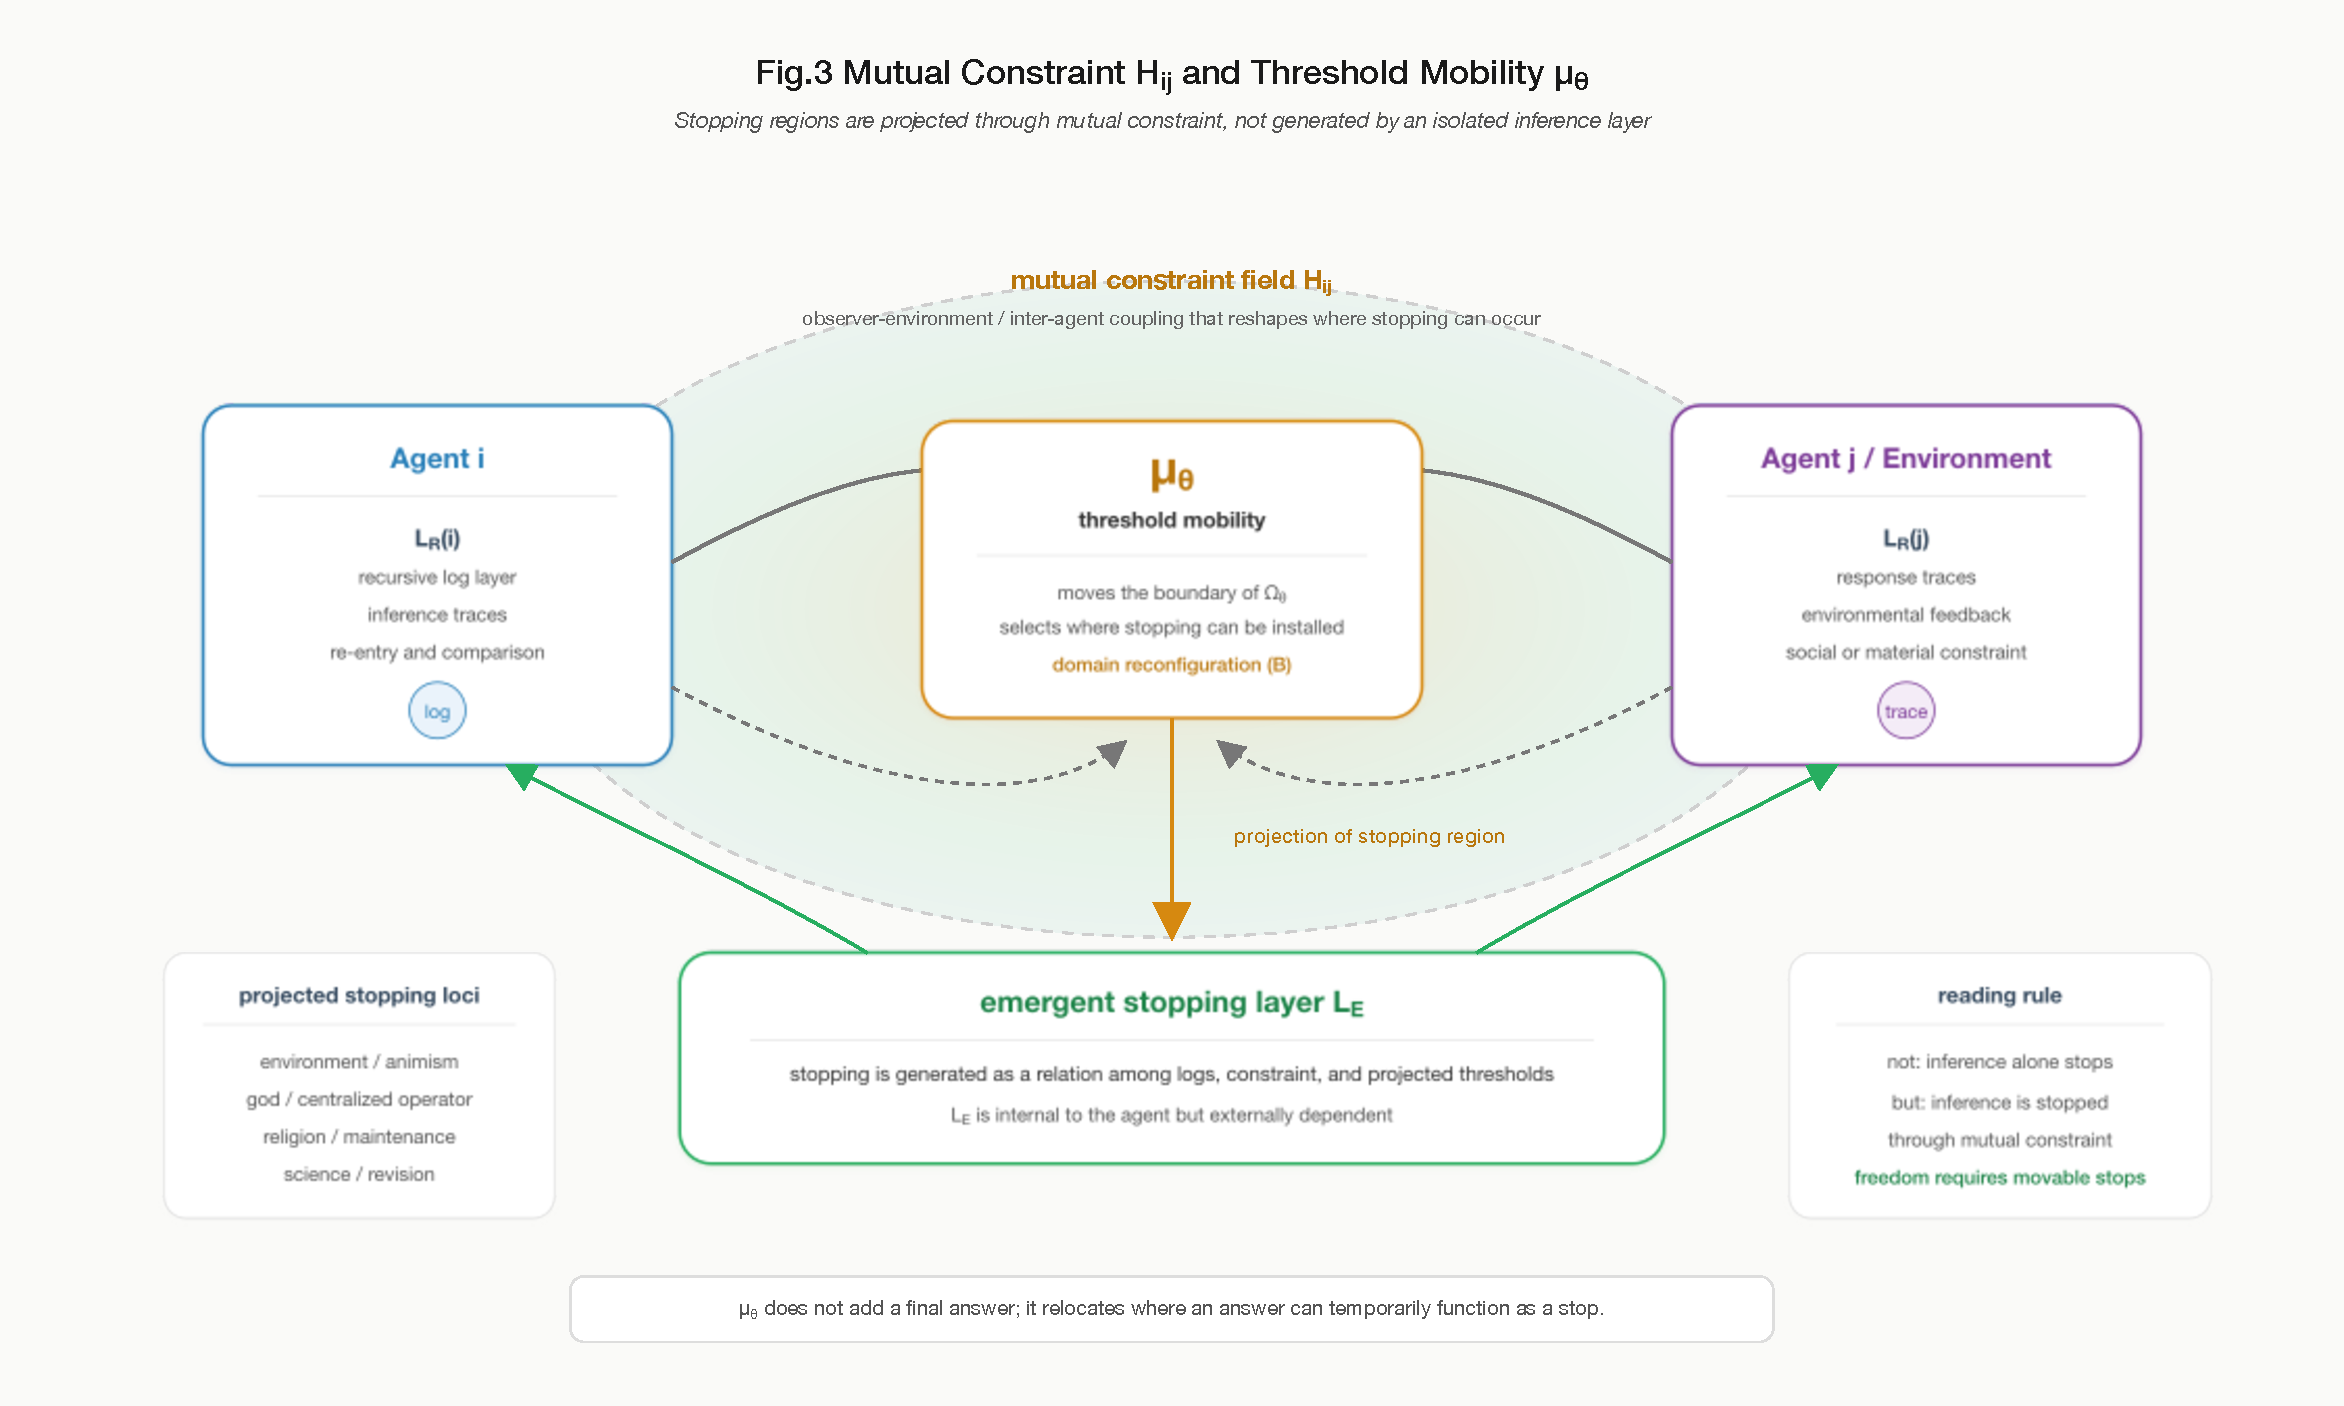
\includegraphics[width=\linewidth]{fig3_mutual_constraint_mu_theta.pdf}
\caption{Mutual constraint $H_{ij}$ and threshold mobility $\mu_\theta$. Projection of stopping regions through mutual constraint is a mechanism hypothesis, not an executed result.}
\label{fig:part2-mutual-constraint}
\figurenote{$H_{ij}$ is hypothesized to affect possible stopping sites. $\mu_\theta$ names mobility in the proposed installation-region account for the stopping operator $E$.}{Stopping is placed outside the modeled action of $L_F$. Its projection and emergence as $L_E$ through the relation between $L_R$ and $H_{ij}$ remain hypotheses. Movable stopping is proposed to support revisable inference, not established subjective freedom.}
\end{figure}

\noindent\textbf{Historical architecture figure.} The next three-layer figure preserves the old-model architecture hypothesis. Its inference/no-fixed-point/cannot-stop chain refers to the historical state-map/justification model, not the active realized-record/position contract. The depicted trace-to-stopping-layer chain remains a hypothesis, not a proof of formation, autonomous own-layer capacity, or a chosen system boundary. The caption and asset are retained with their existing holds.

The next figure, including its caption and footer, is retained legacy architecture, not a diagram of the active support, role, and regime account. Its three boxes are not new formal object types; the stable basin is not evidence for LE, and the trace-to-layer arrow is not a promotion law. Neither its no-fixed-point label nor its Transformer footer certifies a current role or present-day capability under the three analytical boundaries below. The temporary scaffold regime described below must not be mentally added as a fourth box. The mobility and convergence channel remains the old unestablished mechanism, not a new role-assessment rule.

\begin{figure}[H]
\centering
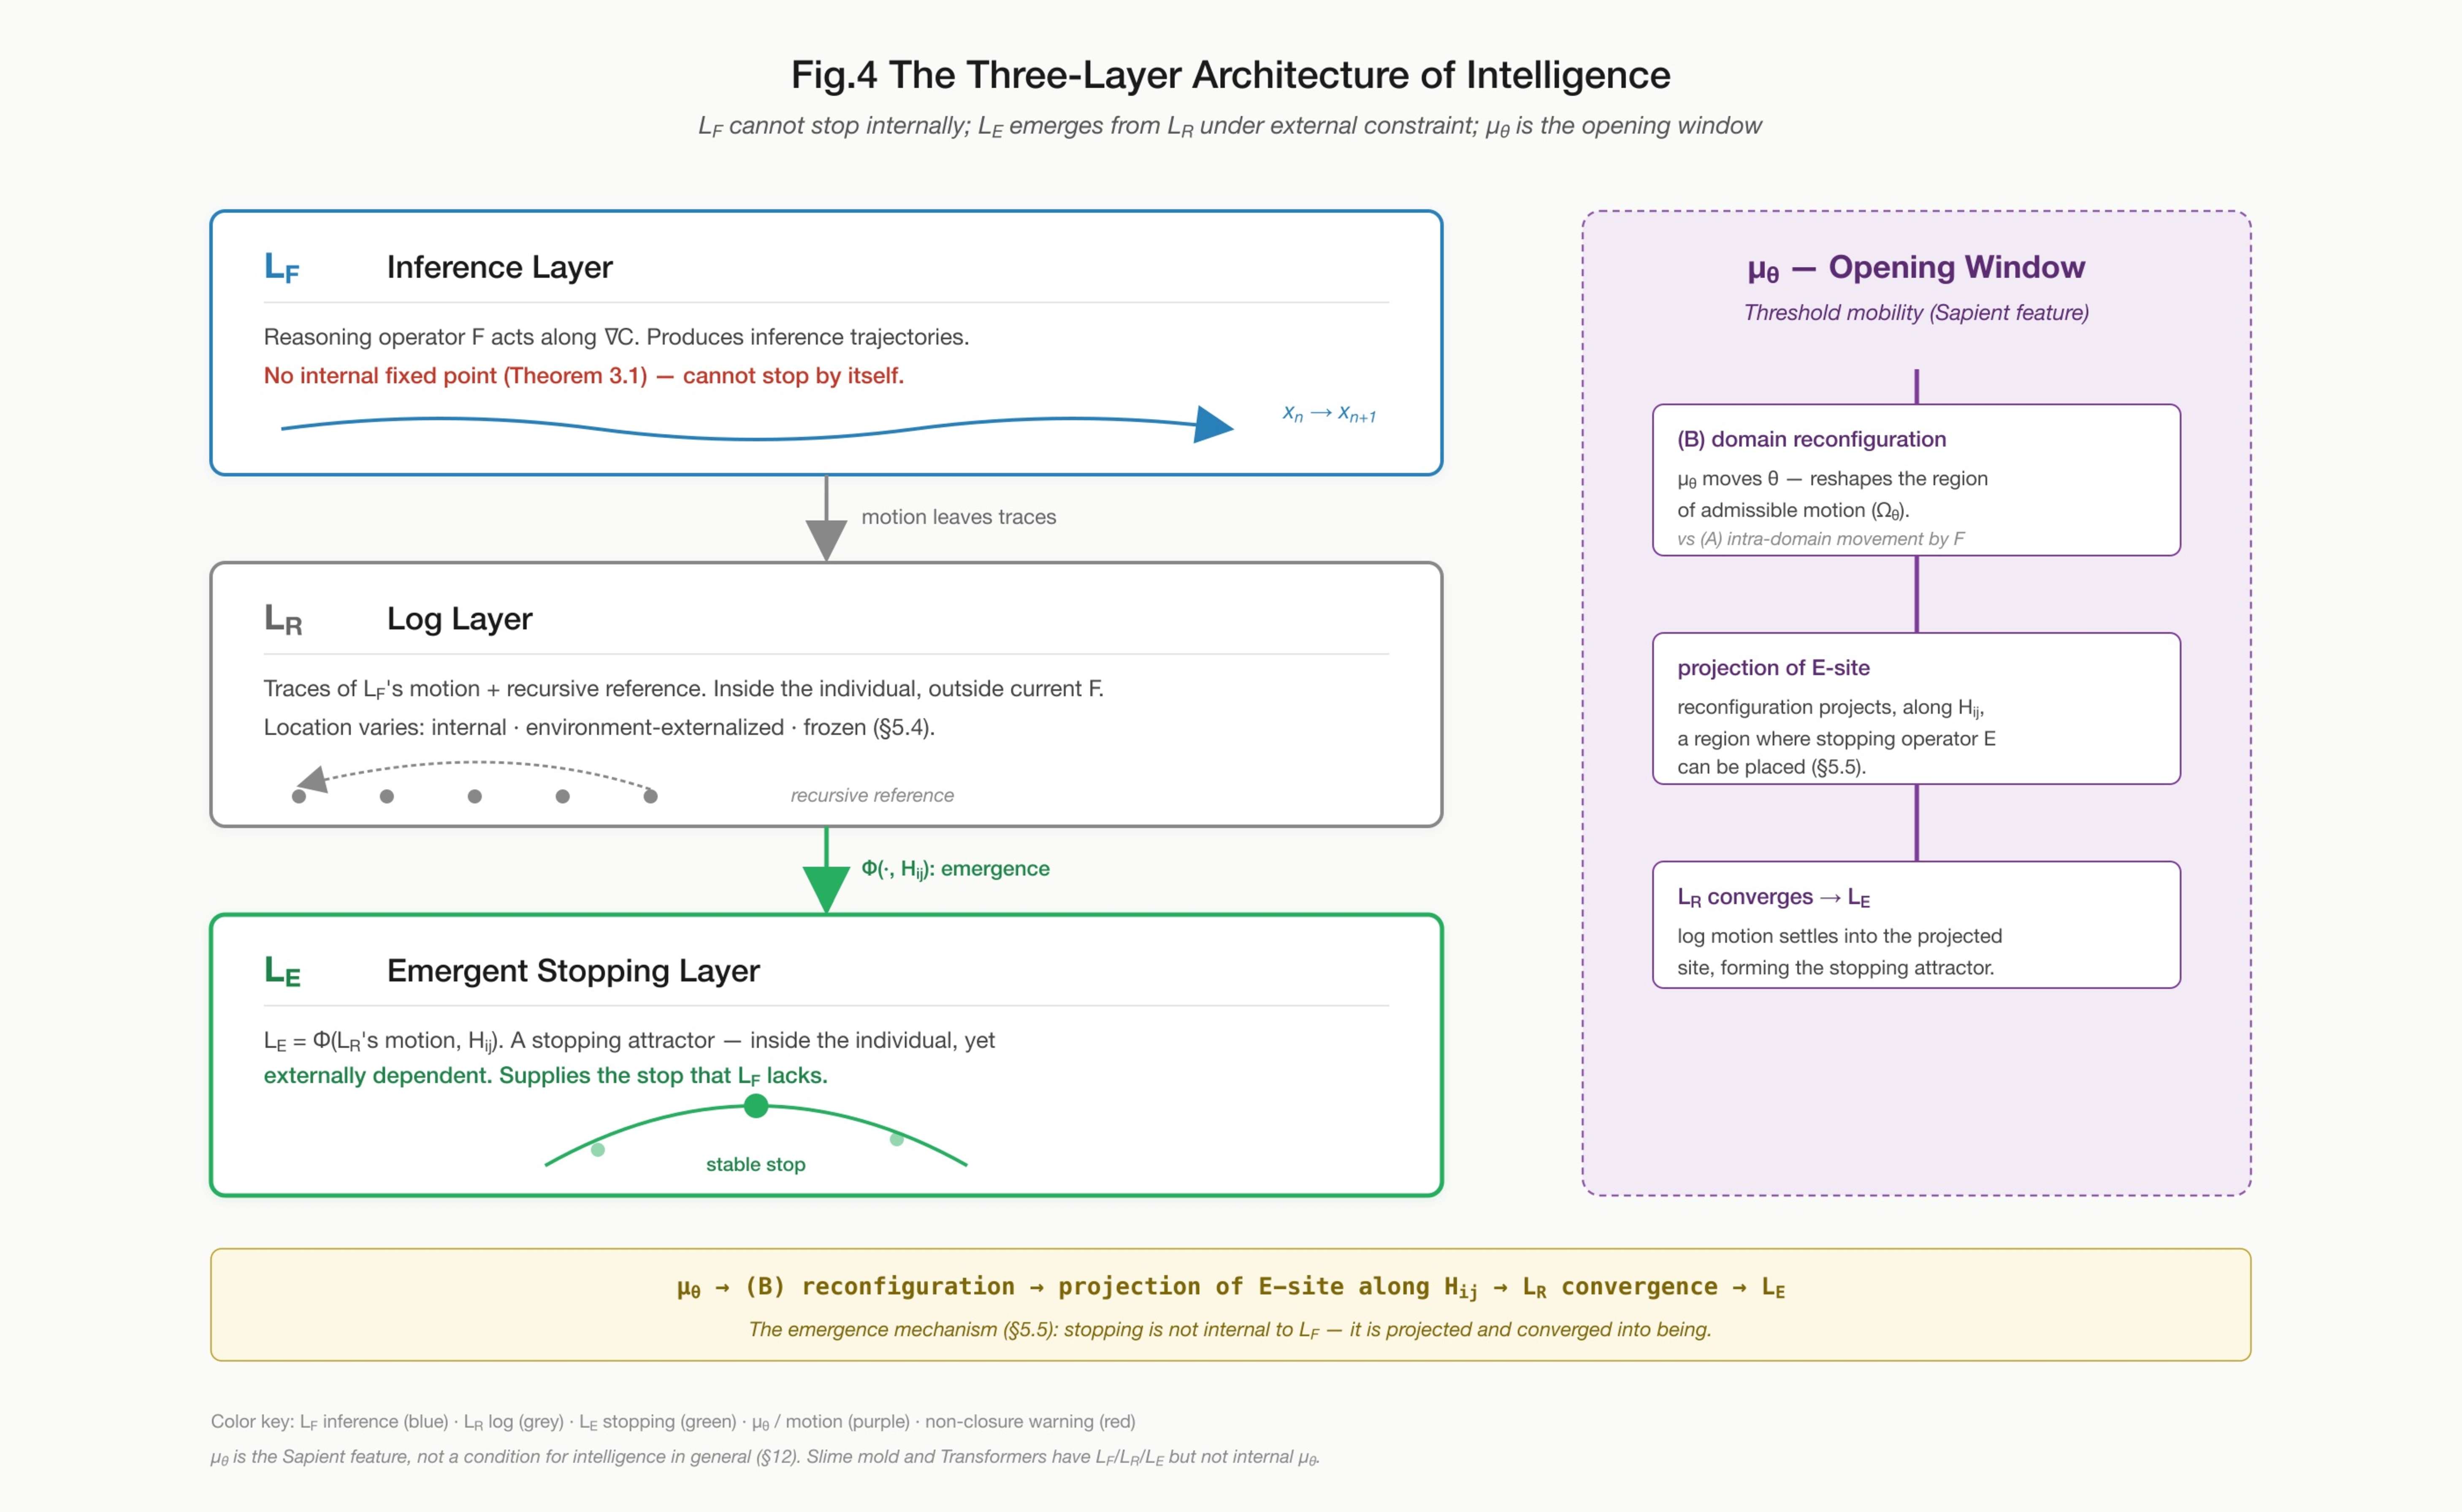
\includegraphics[width=\linewidth]{fig4_three_layer_architecture.pdf}
\caption{The proposed model-local three-layer architecture. The assigned roles are $L_F$, $L_R$, and $L_E$; $\mu_\theta$ is the opening window through which stopping regions can be reconfigured.}
\label{fig:part2-three-layer}
\figurenote{$L_F$ lacks an internal fixed point under the stated conditional stopping model. Its motion leaves traces in $L_R$, and recursive log motion under $H_{ij}$ is hypothesized to be related to $L_E$; independent detection remains open.}{The figure joins the two centers of the paper: non-closure in \S{}3 and emergent stopping in \S{}5. The limit of $L_F$ does not by itself establish higher-layer formation. The own-layer/whole-system boundary remains unresolved.}
\end{figure}

\subsection{Problem Setting}

Real intelligence stops. Humans end a chain of reasoning, make judgments, and act. The historical local-state model's conditional result of \S{}3 does not decide the source of all observed stopping; the proposal here places stopping outside the modeled action of $L_F$. The question is what ``elsewhere'' means.

The proposal assigns a stopping role to a layer modeled as internal to the individual but externally dependent: the emergent stopping layer $L_E$. This assignment does not establish the existence or independent detection of the layer.

\subsection{The Log Layer $L_R$}

The next two paragraphs, ending with logs existing individually and socially, retain the historical log-layer account of recursive-reference processes and their proposed locations. They do not identify a whole process or layer with a single retention support. The active retained-trace role is specified immediately after that preserved account.

The log layer $L_R$ is the layer of recursive reference to traces left by inference. These traces include passed states, attempted branches, failed paths, and points of divergence. $L_R$ is inside the individual in many systems, but outside the current operation of $F$.

The location of $L_R$ differs by system. In a slime mold, logs can be externalized into the environment as slime traces. In a Transformer, training data are frozen logs and context tokens are volatile logs. In sapiens-like intelligence, logs exist both individually and socially.

The preserved log-layer account ends here. In the active account, LR names the registered or retained-trace role of a tracked support, in principle re-referenceable under the declared scope and window. Recursive reference is a process involving that support, not the support itself. A trace is not all generated history, and LR is neither the old scalar justification nor the active generative-position port. Support persistence, current accessibility, and currently surfaced history are distinct. Inaccessibility is not support loss; uncertain continuity or access remains Unknown. Copies, transformations, composites, and resurfacing require their own tracking grounds rather than identity inferred from matching content.

The prose name LE' denotes a temporary scaffold regime of the same LR support when it bridges temporal layers in current updating, with reuse and a feedback path assessed for the declared recipient and window. It is not an independent type, object, or additional layer. The LR role alone certifies neither this scaffold regime nor LE. Reassessment can describe weakening, stabilization toward a quasi-stable role, access loss, support loss, or resurfacing; a quasi-stable role can also weaken toward a temporary scaffold. These are possible assessment histories, not a universal progression, threshold rule, promotion operation, or inverse map. Ownness remains a separate descriptor bundle.

\subsection{Definition of $L_E$}

The following numbered definition, emergence schema, internal/external description, and three-example figure are preserved historical architecture, through the end of that figure. They do not define the active support-role contract or certify an attractor. The current quasi-stable retention role is stated after this preserved block.

\textbf{Definition 5.1 (Emergent stopping layer).}
The emergent stopping layer $L_E$ names a stopping-function role, with a separate hypothesized dependence on recursive motion of $L_R$ and external mutual constraint $H_{ij}$:
\[
L_E=\Phi(L_R\text{ motion},H_{ij}).
\]
It is internal to the agent but externally dependent.

\begin{figure}[H]
\centering
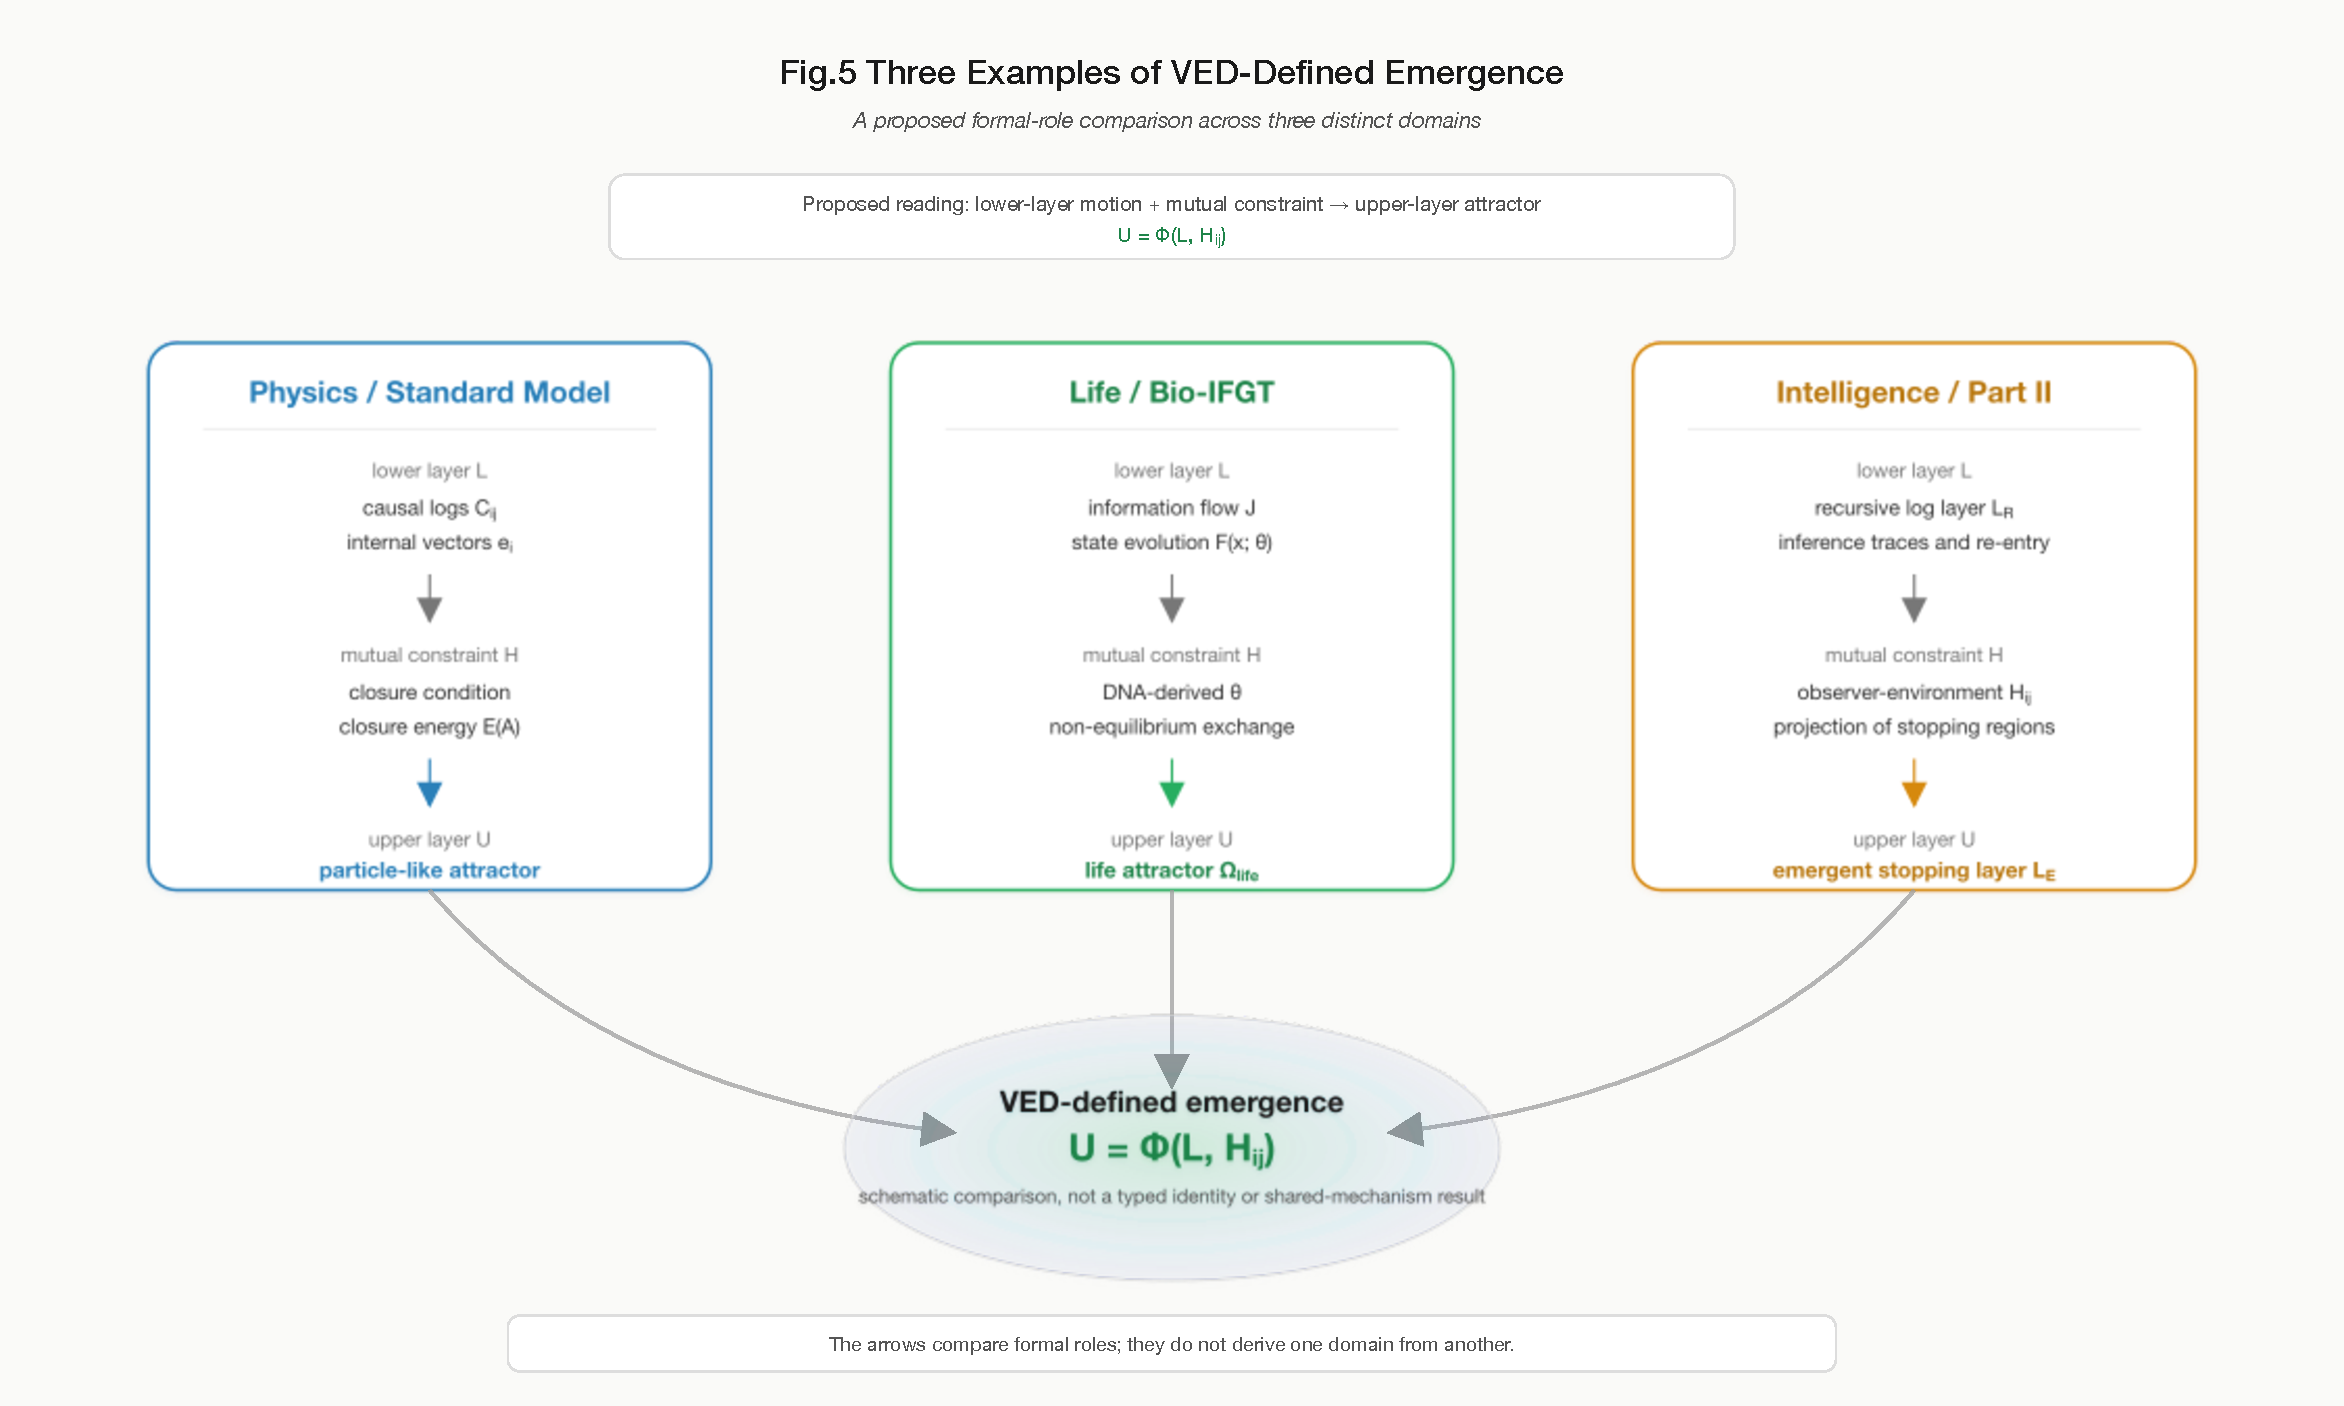
\includegraphics[width=\linewidth]{fig5_three_examples_of_emergence.pdf}
\caption{Three examples placed in a proposed VED comparison of emergence across distinct domains.}
\label{fig:part2-emergence-examples}
\figurenote{Particle-like attractors, the proposed life attractor $\Omega_{\text{life}}$, and the stopping layer $L_E$ are arranged as formal-role analogies around $U=\Phi(L,H_{ij})$.}{The comparison is not an identity, derivation, or typed translation among their objects, carriers, or dynamics.}
\end{figure}

The preserved definition and comparison block ends here. In the active account, LE is a quasi-stable retention role of a tracked support for a declared scope, recipient, and time window, not a permanent store or a proved attractor. A positive model-local assessment requires independently stated grounds for support continuity and trace retention, re-referenceability, role stability under the declared conditions, and feedback availability to that recipient's current updating. This availability is a necessary direction of the scoped role claim, not a sufficient condition or proof of an actual effect. Unestablished criteria remain Unknown; an assignment resting on assumptions is conditional. Long persistence, high reuse, a large iteration count, one feedback event, the old no-fixed-point result, or a figure do not independently certify LE. Calling a support LE because stopping occurred and then explaining that stopping by LE would be circular. This role account supplies no existence, formation, convergence, stopping, autonomy, or ownness theorem; accessibility, control, external dependence, and feedback persistence remain separate assessments.

\subsection{Three Profiles}

Three systems clarify the variability of $L_R$, $\mu_\theta$, and $L_E$.

For the role assignments in the profiles that follow, distinguish three analytical scopes: B1, Transformer-only with a specified invocation and visible input/history representation; B2, model plus runtime or agent system, including its declared storage, retrieval, and controller; B3, human-tool or shared-environment system. In each scope, identify or leave Unknown the recipient, retention and stopping responsibilities, re-entry path, and update-rule responsibility. Runtime memory is not model-native memory, system-level retention is not Transformer own LE, and shared support is not AI autonomy. Expanding a boundary does not create a subject, and artifact origin does not determine ownership. The profiles through the start of the proposed-emergence subsection retain historical or conditional architecture comparisons, not supported presence or absence judgments under the active criteria. This boundary does not rewrite their empirical content or the local mobility definition; it prevents those comparisons from certifying the new roles.

\textbf{Slime mold.} Its logs are environmental; its stopping is interpreted through direct environmental interaction; its $\mu_\theta$ is largely fixed.

\textbf{Transformer.} Its logs are internalized as frozen weights and volatile context; its stopping is externally injected through EOS tokens, task specifications, or decoding controls; it does not generate its own $L_E$ in the sense used here.

\textbf{Sapiens.} Logs are both individual and social; $L_E$ is proposed as an internal, socially related role; $\mu_\theta$ can be moved endogenously.

\subsection{Proposed Emergence Mechanism}

From the next paragraph through the end of the Projection subsection, the stages, arrows, and projection comparisons retain the old, unexecuted mechanism hypothesis. They are not the active support-role criteria or a transition law for the temporary scaffold regime. In particular, log convergence does not certify the current LE role. This enclosure leaves the local threshold-mobility definition and the comparison with the consciousness paper intact; it supplies no E or field mechanism.

The emergence of $L_E$ is hypothesized through four schematic stages, not an executed process:
\begin{enumerate}
\item $\mu_\theta$ causes region reconfiguration (B);
\item the reconfiguration projects a possible installation region for the stopping operator $E$;
\item the recursive motion of $L_R$ converges into the projected region;
\item the resulting stable stopping attractor is $L_E$.
\end{enumerate}

Schematically:
\[
\mu_\theta \to (B)\text{ reconfiguration} \to E\text{-region projection} \to L_R\text{ convergence} \to L_E .
\]

This mechanism hypothesis relates movable stopping to a functional reading of free inference; it is not an explanation of subjective freedom. A relation between absent stopping resources and unsustainable branching or regress is hypothesized. $L_E$ is proposed as a functional resource for finite inference, not shown to emerge for the purpose of sustaining freedom.

\subsection{Projection}

The projection used here is compared by role with the projection primitive in the consciousness paper; a shared typed operator is not established. It means that a state or relation acquires unequal influence within a field. In this paper, the projected object is a possible stopping locus.

\subsection{External Stopping Operator}

\noindent\textbf{Preserved historical notation.} The following action definition, non-membership display, and externality explanation are retained old-model material, ending before the next field/network subsection. The active optional successor adapter is not substituted into the old iteration family. The type of E remains unresolved; this block establishes neither internal non-derivability nor noncomputability, and a large iteration count alone does not establish E. No E operator is formalized here.

The external stopping operator $E$ is the action of $L_E$ on an inferential state:
\[
E=E[L_E,x_n],\qquad E\notin\{F^k\}.
\]
It is external because it is not a member of the sequence of inference operations. It acts through $L_E$.

\subsection{$\Phi_{\text{ext}}\equiv\Phi_{\text{net}}$}

The external reference field $\Phi_{\text{ext}}$ is compared as a proposed second view with the inter-individual network of emergent stopping layers $\Phi_{\text{net}}$:
\[
\Phi_{\text{ext}}\equiv\Phi_{\text{net}}.
\]
Here $\Phi_{\text{ext}}$ should be read as an intelligence-layer projection of the IFGT potential vocabulary, not as the full IFGT field itself. It names the way a shared stopping structure appears as an external reference field from within an individual inference window.

\begin{figure}[H]
\centering
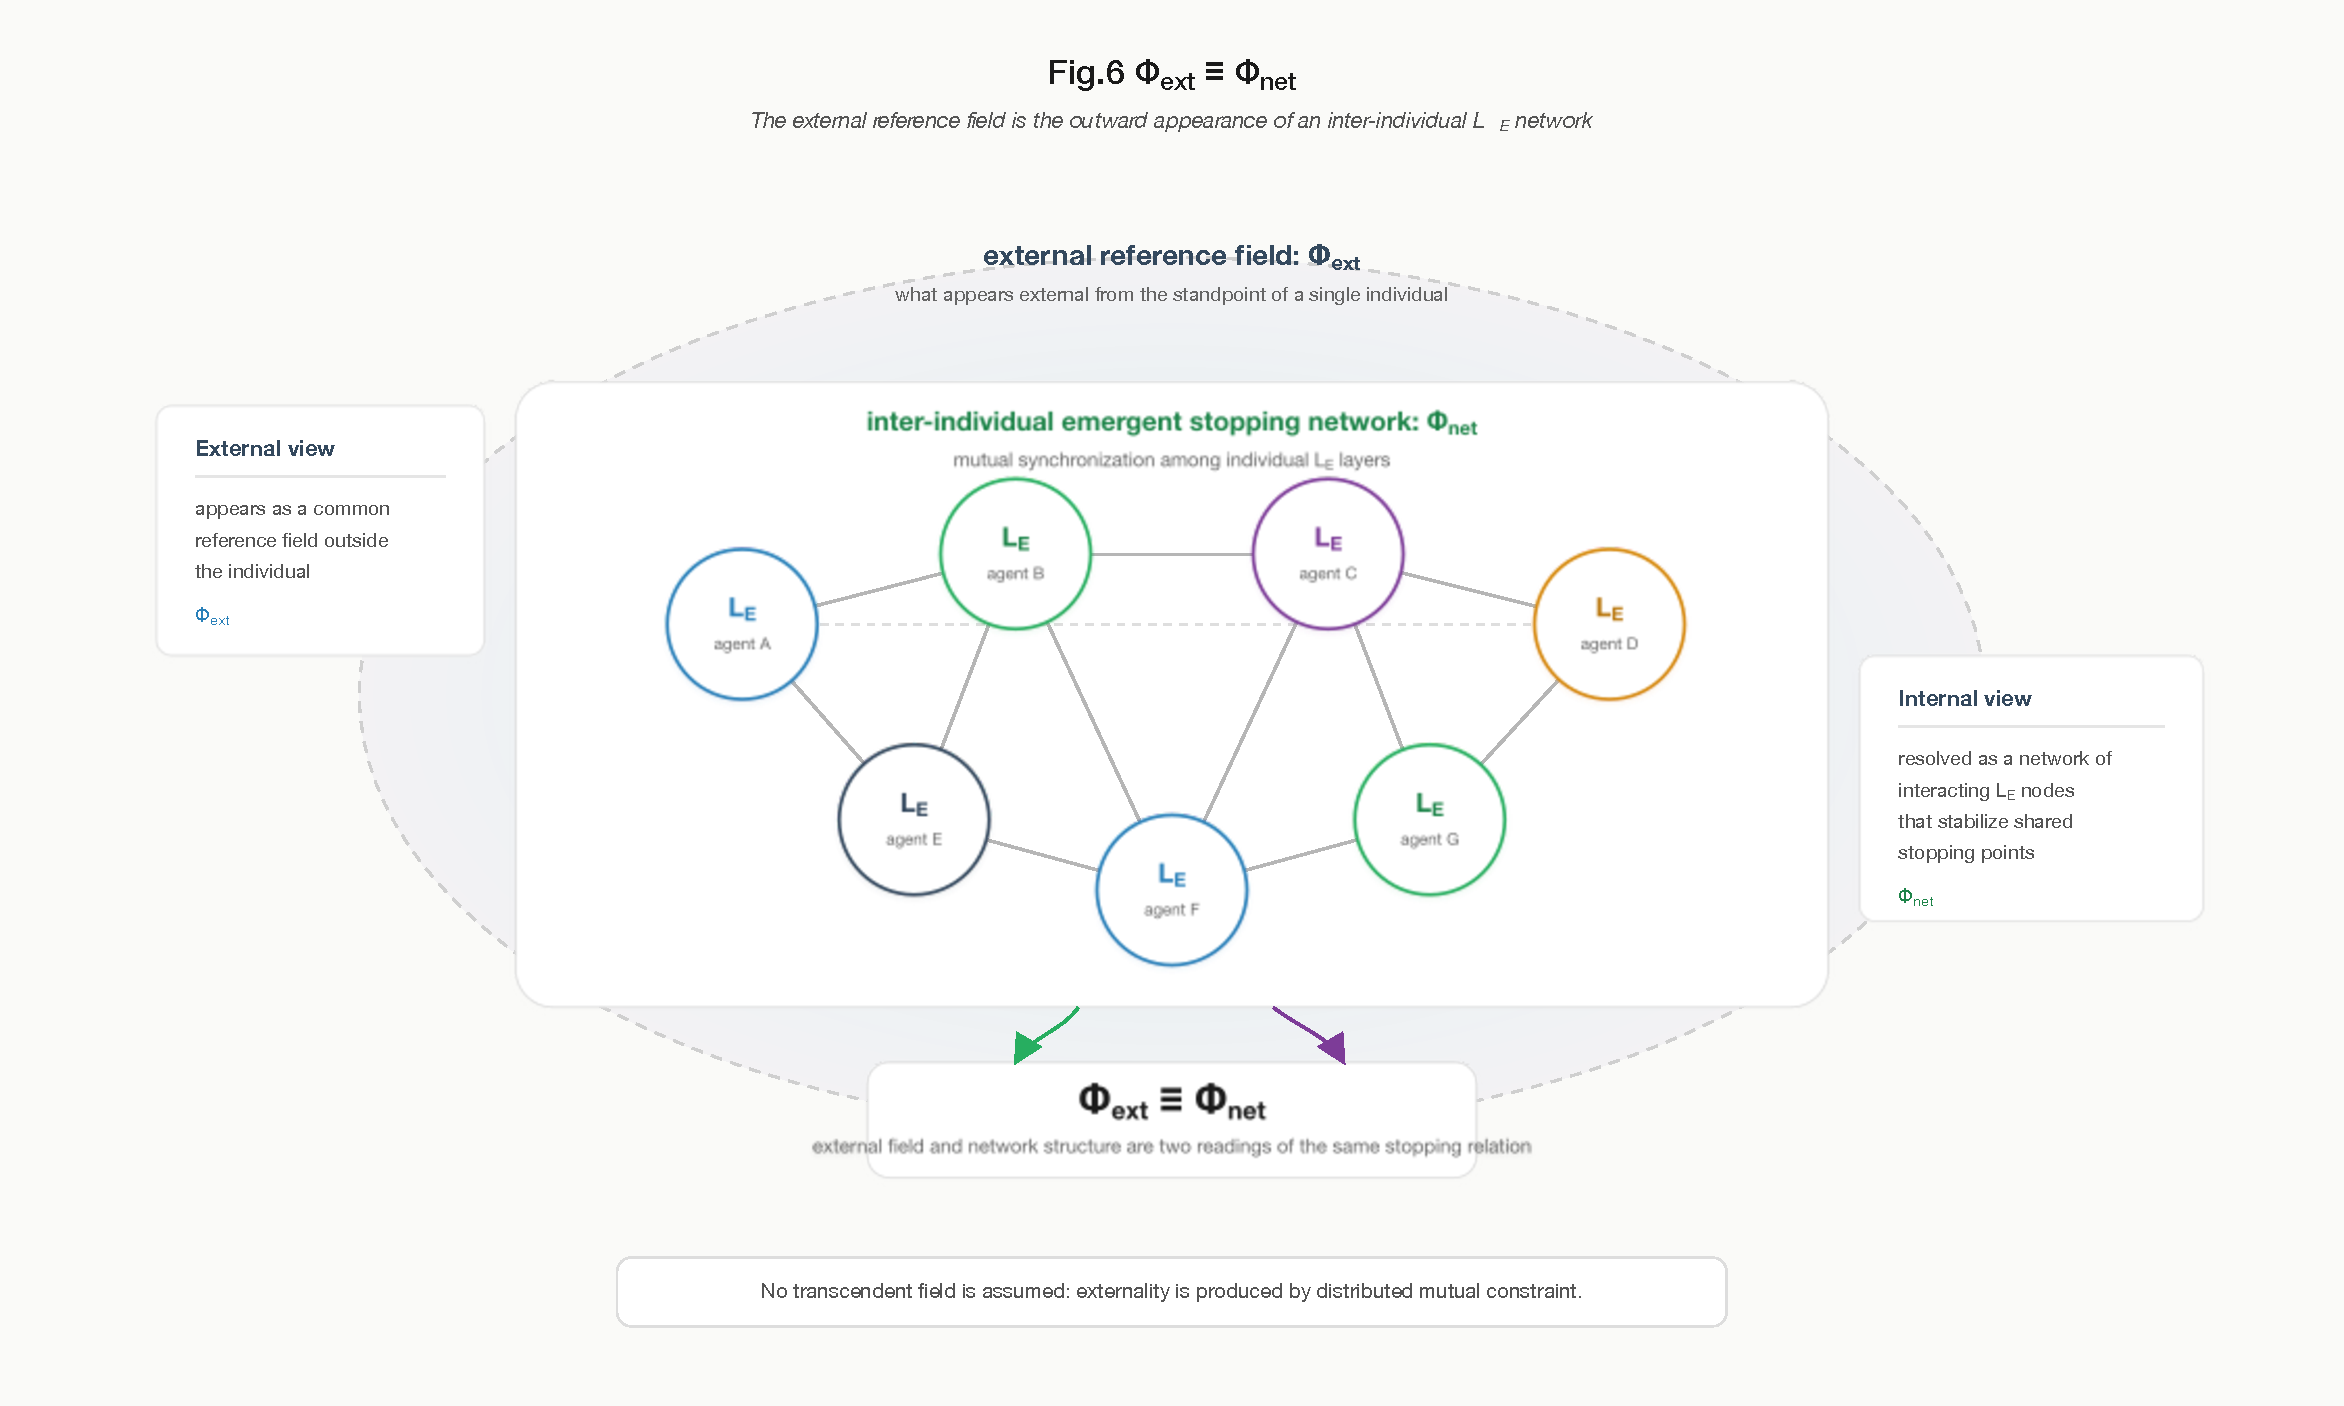
\includegraphics[width=\linewidth]{fig6_phi_ext_phi_net.pdf}
\caption{$\Phi_{\text{ext}} \equiv \Phi_{\text{net}}$. The retained identity notation is unresolved. External reference and the network of individual $L_E$ layers are proposed as two views, not established as identical.}
\label{fig:part2-phi-ext-net}
\figurenote{$\Phi_{\text{ext}}$ is the external appearance; $\Phi_{\text{net}}$ is the internal network structure of mutually synchronized $L_E$ layers.}{No transcendent field needs to be assumed. Norms, gods, truth, and monetary value can be read as appearances of distributed $L_E$ synchronization.}
\end{figure}

The preceding E and field/network blocks remain in their preserved scope. The active support-role account neither types E nor repairs the field/network identity or supplies a co-formation map. Re-reference and re-entry are not by themselves effective return; role assignment is neither synchronization nor a guarantee of recovery or revisability. The optional inference adapter is not substituted into the old iteration notation.

\subsection{Summary}

The proposed architecture relates $L_F$, $L_R$, and $L_E$ under externally dependent stopping; its generation and persistence claims remain hypotheses. Sapiens-like intelligence adds endogenous $\mu_\theta$, allowing stopping loci to be reorganized rather than merely received.

The active architectural contribution is the scoped account of a tracked support's registered-trace role, temporary scaffold regime, and quasi-stable retention role, with distinct evidence statuses and feedback descriptors. The preceding layer definition and generation account remain preserved proposals, not consequences proved by these roles. Stopping, formation, and rule change retain their separate burdens; the current account does not make the whole chapter historical.

\bigskip
